\documentclass{article}

\usepackage{fancyhdr}
\usepackage{extramarks}
\usepackage{amsmath}
\usepackage{amsthm}
\usepackage{amsfonts}
\usepackage{empheq}
\usepackage{mathtools}
\usepackage{physics}
\usepackage{hyperref}
\usepackage[dvipsnames]{xcolor} 
\hypersetup{
	colorlinks,
	linkcolor=BrickRed,
}
\usepackage{tikz}
\usetikzlibrary {datavisualization.formats.functions}
\usepackage{graphicx}
\usepackage{subcaption}
\usepackage{neuralnetwork}
\usepackage{comment}


\newcommand\numberthis{\addtocounter{equation}{1}\tag{\theequation}}

%
% Basic Document Settings
%

\topmargin=-0.45in
\evensidemargin=0in
\oddsidemargin=0in
\textwidth=6.5in
\textheight=9.0in
\headsep=0.25in

\linespread{1.2}

\pagestyle{fancy}
\lhead{\hmwkAuthorName}
\chead{\hmwkClass: \hmwkTitle}
\rhead{\firstxmark}
\lfoot{\lastxmark}
\cfoot{\thepage}

\renewcommand\headrulewidth{0.4pt}
\renewcommand\footrulewidth{0.4pt}

\setlength\parindent{0pt}

%
% Create Question Sections
%

\newcommand{\enterQuestionHeader}[1]{
	\nobreak\extramarks{}{Question \arabic{#1} cont'd on next page\ldots}\nobreak{}
	\nobreak\extramarks{Question \arabic{#1} (cont'd)}{Question \arabic{#1} cont'd on next page\ldots}\nobreak{}
}

\newcommand{\exitQuestionHeader}[1]{
	\nobreak\extramarks{Question \arabic{#1} (cont'd)}{Question \arabic{#1} cont'd on next page\ldots}\nobreak{}
	\stepcounter{#1}
	\nobreak\extramarks{Question \arabic{#1}}{}\nobreak{}
}

\setcounter{secnumdepth}{0}
\newcounter{partCounter}
\newcounter{homeworkQuestionCounter}
\setcounter{homeworkQuestionCounter}{1}
\nobreak\extramarks{Question \arabic{homeworkQuestionCounter}}{}\nobreak{}

%
% Homework Question Environment
%
% This environment takes an optional argument. When given, it will adjust the
% problem counter. This is useful for when the problems given for your
% assignment aren't sequential. See the last 3 problems of this template for an
% example.
%
\newenvironment{homeworkQuestion}[1][-1]{
	\ifnum#1>0
	\setcounter{homeworkQuestionCounter}{#1}
	\fi
	\section{Question \arabic{homeworkQuestionCounter}}
	\rule{0.9\textwidth}{3pt}\\
	\setcounter{partCounter}{1}
	\enterQuestionHeader{homeworkQuestionCounter}
}{
	\exitQuestionHeader{homeworkQuestionCounter}
}

%
% Homework Details
%   - Title
%   - Due date
%   - Class
%   - Section/Time
%   - Instructor
%   - Author
%

\newcommand{\hmwkTitle}{HW\#13}
\newcommand{\hmwkDueDate}{}
\newcommand{\hmwkClass}{CpE 520}
\newcommand{\institute}{West Virginia University}
\newcommand{\hmwkClassInstructor}{Professor Nasser Nasrabadi}
\newcommand{\hmwkAuthorName}{\textbf{Ali Zafari}}

%
% Title Page
%

\title{
	\vspace{2in}
	\textmd{\textbf{\hmwkClass:\ \hmwkTitle}}\\
	\vspace{0.1in}\large{\institute}\\
%	\vspace{0.1in}\large{\textit{\hmwkClassInstructor}}
	\vspace{3in}
}

\author{\hmwkAuthorName}
\date{}

\renewcommand{\part}[1]{\textbf{\Large Part \Alph{partCounter}}\stepcounter{partCounter}\\}

\begin{document}
	
	\pagenumbering{gobble}% prevent cover page of numbering
	\maketitle
	\pagebreak % let cover page free to the end of page
	\pagenumbering{arabic} % start page numbering again from 1 and print them!

	
	
	\begin{homeworkQuestion}%Question 1
		\subsection{Part (a): Inverse of $\mathbf{y_{n\times1}=A_{n\times m}x_{m\times 1}}$ where n<m and rank=n }
		In this case there are more unknowns than equations so the system is underdetermined. Because the matrix $A$ is full rank with $rank=n$, $AA^T$ will be an $n\times n$ non-singular square matrix. Therefore, there will be an inverse for it like below:
		\begin{equation*}
		(AA^T)(AA^T)^{-1}  = I
		\tag{*}
		\end{equation*}
		As it is clear from the above equation, we may use $A^T(AA^T)^{-1}$ as a right inverse for matrix $A$. We first assume that the inverse we are seeking for has an equation like  $\mathbf{x_{m\times 1}=R_{m\times n}y_{n\times1}}$. Finding $R_{m\times n}$ will be the goal. We propose $R_{m\times n} = A^T(AA^T)^{-1}$ and through the equations below we will check if it will result in our main equation:
		\begin{empheq}[box=\fbox]{equation*}
		\mathbf{x}\mathbf{=A^T(AA^T)^{-1}y}
		\end{empheq}
		\begin{align*}
		\mathbf{x}&\mathbf{=A^T(AA^T)^{-1}y}\\
		\xrightarrow{\times A}\mathbf{Ax}&=\mathbf{AA^T(AA^T)^{-1}y}\\
		\xrightarrow{\text{using *}}\mathbf{Ax}&=\mathbf{y}
		\end{align*}
		\rule{0.2\textwidth}{0.5pt}
		
		\subsection{Part (b): Inverse of $\mathbf{y_{n\times1}=A_{n\times m}x_{m\times 1}}$ where n>m and rank=m}
		In this case there are more equations than unknowns, so the system is overdetermined. Because the matrix $A$ is full rank with $rank=m$, $A^TA$ will be an $m\times m$ non-singular square matrix. Therefore, there will be an inverse for it like below:
		\begin{equation*}
		(A^TA)^{-1}(A^TA)  = I
		\tag{**}
		\end{equation*}
		As it is clear from the above equation, we may use $(A^TA)^{-1}A^T$ as a left inverse for matrix $A$. 
		\begin{align*}
		\mathbf{Ax}&\mathbf{=y}\\
		\xrightarrow{\times A^T}\mathbf{A^TAx}&\mathbf{=A^Ty}\\
		\xrightarrow[\text{using *}]{\times (A^TA)^{-1}}\;\;\;\;\;\;\;\;\;\mathbf{x}&\mathbf{=(A^TA)^{-1}A^Ty}
		\end{align*}
		\begin{empheq}[box=\fbox]{equation*}
		\mathbf{x}\mathbf{=(A^TA)^{-1}A^Ty}
		\end{empheq}
	\end{homeworkQuestion}
	\pagebreak
	
	
	\begin{homeworkQuestion}%Question 2
		\subsection{Part (a): Difference Between Ridge and LASSO Regressions}
		Ridge regression uses the the sum of squared values of unknown parameters; however, LASSO regression uses sum of the absolute values of unknown parameters. Therefore, LASSO is capable to make some of the unknown coefficients zero. On the other hand, Ridge regression is able to make the coefficient really small but not absolutely zero.\\ 
		\rule{0.2\textwidth}{0.5pt}
		
		\subsection{Part (b): Expressions for Ridge and LASSO Regressions}
		Ridge Regression:
		\begin{equation*}
			 \mathbf{\tilde{x}=\min_{x} \{(y-Ax)^2+\lambda\sum_{i=1}^{m}}x_i^2\}
		\end{equation*}
		LASSO Regression:
		\begin{equation*}
		\mathbf{\tilde{x}=\min_{x} \{(y-Ax)^2+\lambda\sum_{i=1}^{m}}|x_i|\}
		\end{equation*}
	\end{homeworkQuestion}
	
	
	\begin{homeworkQuestion}%Question 3
		Convolution of two vectors:
		\begin{equation*}
		\begin{bmatrix}
		1\\2\\2\\1
		\end{bmatrix}
		*\begin{bmatrix}
		1&1&1
		\end{bmatrix}
		=\begin{bmatrix}
		1\\1+2\\1+2+2\\2+2+1\\2+1\\1
		\end{bmatrix}
		=\begin{bmatrix}
		1\\3\\5\\5\\3\\1
		\end{bmatrix}
		\end{equation*}
		
	\end{homeworkQuestion}
	
	
	\begin{homeworkQuestion}%Question 4
		
		By using 1x1 convolution in DNNs we can change the depth of channels of a layer so there will be much less computations for the DNN to be trained.
		We can mention an example here to clarify its purpose:\\\\
		Example 1:  input (256 channels) -> 1x1 convolution (64 channels) -> 4x4 convolution (256 channels)\\
		Example 2:  input (256 channels) -> 4x4 convolution (256 channels)\\\\

		If we accept that the computation cost is proportional to the number of weights, we can find it for both the examples above:
		
		number of weights for example 1: 
		\begin{equation*}
			(256 \times 64 \times 1 \times 1) + (64 \times 256 \times 4 \times 4) = 278,528
		\end{equation*}
		
		\begin{equation*}
			256 \times 256 \times 4 \times 4 = 1,048,576
		\end{equation*}
	\end{homeworkQuestion}
	
	
	
	\begin{homeworkQuestion}%Question 5
		
		\begin{itemize}
			\item \textbf{Average Pooling}\\
			It computes the average of the values in its filter.
			\item \textbf{Global Average Pooling}\\
			This layer will compute the average over any channel of the input individually.
			\item \textbf{Max Pooling}\\
			It chooses a single maximum value in its filter.
			
		\end{itemize}
	\end{homeworkQuestion}
	
	
	
	\begin{homeworkQuestion} %Question 6
		Softmax Regression is actually a generalization of logistic regression that could be used for multi-class classification, in contrast of what we have in logistic regression which classifies between two classes.
	\end{homeworkQuestion}
	
	
	\begin{homeworkQuestion} %Question 7
		Hinge loss expression:
		\begin{equation*}
			L(d, y) = max(0, 1 - dy)
		\end{equation*}
		in which $d$ is the desired response and $y$ is the computed output by the SVM.\\\\
		This loss function is mainly used in support vector machines (SVM).
	\end{homeworkQuestion}
	\pagebreak
	
	\begin{homeworkQuestion} %Question 8
		\par 
		L1 norm:
		\begin{equation*}
		\mathbf{||x||_1} = \sum_{i=1}|x_i|
		\end{equation*}
		L2 norm:
		\begin{equation*}
		\mathbf{||x||_2} = \sqrt{\sum_{i=1}|x_i|^2}
		\end{equation*}
	\end{homeworkQuestion}
	
	
	\begin{homeworkQuestion} %Question 9
		Two main applications of autoencoders are \textbf{data denoising} and \textbf{dimensionality reduction} for data visualization. An advantage of autoencoders is that they do not require ay engineering to reduce the dimensionality. So, by only providing enough amount of data they could be trained automatically.
	\end{homeworkQuestion}
	\pagebreak
	
	\begin{homeworkQuestion}
		There are three unknown weights to be found on the below neural network, so it can perform XOR operation. 
	\begin{figure*}[h!]
		\centering
		\begin{neuralnetwork}[height=5, nodespacing=2cm, layerspacing=5cm, nodesize=20pt]
			\newcommand{\nodetextclear}[2]{}
			\newcommand{\nodetextxnb}[2]{\ifnum #2=0 $\mathbf{X_0}$ \else\ifnum #2=1 $\mathbf{X_1}$ \else \ifnum #2=2 $\mathbf{X_2}$ \fi \fi \fi}
			\newcommand{\logiclabel}[1]{\,{$\scriptstyle#1$}\,}
			\newcommand{\nodetextH}[2]{\ifnum #2=0 $\mathbf{h_0}$ \else\ifnum #2=1 $\mathbf{h_1}$ \else \ifnum #2=2 $\mathbf{h_2}$ \fi \fi \fi}
			\newcommand{\nodetextY}[2]{$\mathbf{y}$}
			\newcommand{\linklabelsAone}[4]{\ifnum#4=1 $w_{13}=?$ \else $w_{14}=?$ \fi}
			\newcommand{\linklabelsAtwo}[4]{\ifnum#4=1 $w_{23}=?$ \else \logiclabel{-4} \fi}
			\newcommand{\linklabelsBiasIn}[4]{\ifnum#4=1 \logiclabel{-1} \else \logiclabel{-1} \fi}
			\newcommand{\linklabelsBiasHidden}[4]{\logiclabel{-1}}
			\newcommand{\linklabelsY}[4]{\ifnum#2=1 \logiclabel{+2} \else \logiclabel{+2} \fi}
			\inputlayer[count=2, bias=true, text=\nodetextxnb]
			\hiddenlayer[count=2, bias=true, text=\nodetextH]
			\outputlayer[count=3, exclude={1, 3}, text=\nodetextY]
			\link[from layer=0, to layer=1, from node=0, to node=1, label=\linklabelsBiasIn, labelpos=very near start]
			\link[from layer=0, to layer=1, from node=0, to node=2, label=\linklabelsBiasIn, labelpos=very near start]
			\link[from layer=0, to layer=1, from node=1, to node=1, label=\linklabelsAone, labelpos=very near start]
			\link[from layer=0, to layer=1, from node=2, to node=1, label=\linklabelsAtwo, labelpos=very near start]
			\link[from layer=0, to layer=1, from node=1, to node=2, label=\linklabelsAone, labelpos=very near start]
			\link[from layer=0, to layer=1, from node=2, to node=2, label=\linklabelsAtwo, labelpos=very near start]
			\link[from layer=1, to layer=2, from node=0, to node=2, label=\linklabelsBiasHidden]
			\link[from layer=1, to layer=2, from node=1, to node=2, label=\linklabelsY]
			\link[from layer=1, to layer=2, from node=2, to node=2, label=\linklabelsY]
		\end{neuralnetwork}
		\label{fig:xor}
	\end{figure*}


The equation for neurons of the network are written below ($\varphi$ is the threshold function):
	\begin{align*}
		\mathbf{h_1}&\mathbf{=\varphi(w_{13}X_1+w_{23}X_2-1)}\\
		\mathbf{h_2}&\mathbf{=\varphi(w_{14}X_1-4X_2-1)}\\
		\mathbf{y}&\mathbf{=\varphi(2h_1+2h_2-1)}
	\end{align*}
	With calculating the equations of the lines in the $X_1$-$X_2$ coordinate system, all of the weights will be found.	
	\begin{figure*}[h]
		\centering
		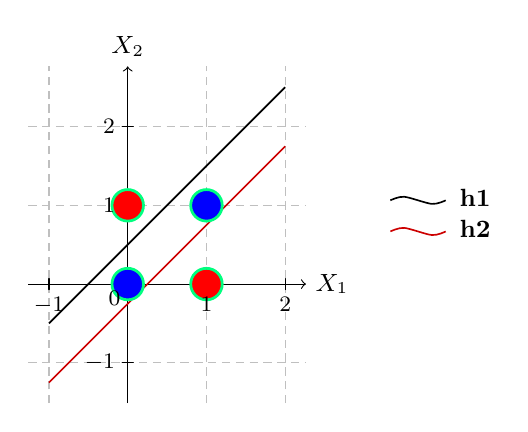
\begin{tikzpicture}
		\datavisualization [school book axes,
		all axes={grid},
		every grid/.append style={style=densely dashed},
		visualize as smooth line/.list={h1,h2},
		style sheet=strong colors,
		h1={label in legend={text=$\mathbf{h1}$}},
		h2={label in legend={text=$\mathbf{h2}$}},
		x axis={label=$X_1$},
		y axis={label=$X_2$},
		data/format=function,]
		data [set=h1] {
			var x : interval [-1:2];
			func y = 0.5 + \value x;
		}
		data [set=h2] {
			var x : interval [-1:2];
			func y = -0.25 + \value x;
		}
		info {
			\filldraw [SpringGreen, fill=blue, line width=1pt] (visualization cs: x=0, y=0) circle [radius=2mm];
			\filldraw [SpringGreen, fill=red, line width=1pt] (visualization cs: x=0, y=1) circle [radius=2mm];
			\filldraw [SpringGreen, fill=red, line width=1pt] (visualization cs: x=1, y=0) circle [radius=2mm];
			\filldraw [SpringGreen, fill=blue, line width=1pt] (visualization cs: x=1, y=1) circle [radius=2mm];
		};
		
		\end{tikzpicture}
		\label{fig:xor_plot}
	\end{figure*} 

	\begin{align*}
		&\mathbf{-2X_1+2X_2-1=0} \rightarrow w_{13}=-2, w_{23}=2\\
		&\mathbf{4X_1-4X_2-1=0} \rightarrow w_{14}=4
	\end{align*}
	\end{homeworkQuestion}
	\pagebreak
	
	\begin{homeworkQuestion} %Question 11
		Derivative of sigmoid function:
		\begin{align*}
		\frac{\partial}{\partial x}f(x)&=\frac{\partial}{\partial x}(\frac{1}{1+e^{-\lambda x}})\\
		&=\frac{\lambda e^{-\lambda x}}{(1+e^{-\lambda x})^2}\\
		&=\lambda (\frac{ e^{-\lambda x}}{1+e^{-\lambda x}})(\frac{1}{1+e^{-\lambda x}})\\
		&=\lambda (\frac{1+e^{-\lambda x}-1}{1+e^{-\lambda x}})(\frac{1}{1+e^{-\lambda x}})\\
		&=\lambda (1-\frac{1}{1+e^{-\lambda x}})(\frac{1}{1+e^{-\lambda x}})\\
		&=\lambda f(x)(1-f(x))
		\end{align*}
	\end{homeworkQuestion}
	
	
	\begin{homeworkQuestion} %Question 12
		Kernel function is a function which with the help of dot product could do the same operation as mapping from input space to a high dimensional output space.\\\\
		Kernel Trick is a way by which we can simply compute the inner products of the input samples (with the help of kernel function) in their own input feature space without any need to compute the mapping explicitly. This operation will be less computationally expensive. 
	\end{homeworkQuestion}
	
	
	\begin{homeworkQuestion} %Question 13
		we start with $\phi(\mathbf{x_i})^T\phi(\mathbf{x_j})$:
		\begin{align*}
		\phi(\mathbf{x_i})^T\phi(\mathbf{x_j}) &=\begin{bmatrix}
		x_{i_1}^2\\ \sqrt{2}x_{i_1}x_{i_2} \\ x_{i_2}^2
		\end{bmatrix}^T \begin{bmatrix}
		x_{j_1}^2\\ \sqrt{2}x_{j_1}x_{j_2} \\ x_{j_2}^2
		\end{bmatrix}\\
		&= x_{i_1}^2x_{j_1}^2 + 2x_{i_1}x_{j_1}x_{i_2}x_{j_2} + x_{i_2}^2x_{j_2}^2\\
		&= (x_{i_1}x_{j_1} + x_{i_2}x_{j_2})^2\\
		&= (\mathbf{x_i^Tx_j})^2\\
		&= k(\mathbf{x_i, x_j})
		\end{align*}
	\end{homeworkQuestion}
	
	

	
\end{document}